\section{Pseudo Labeling}
\label{sec:labeling}
% \begin{figure}[!htb]
%     \centering
%     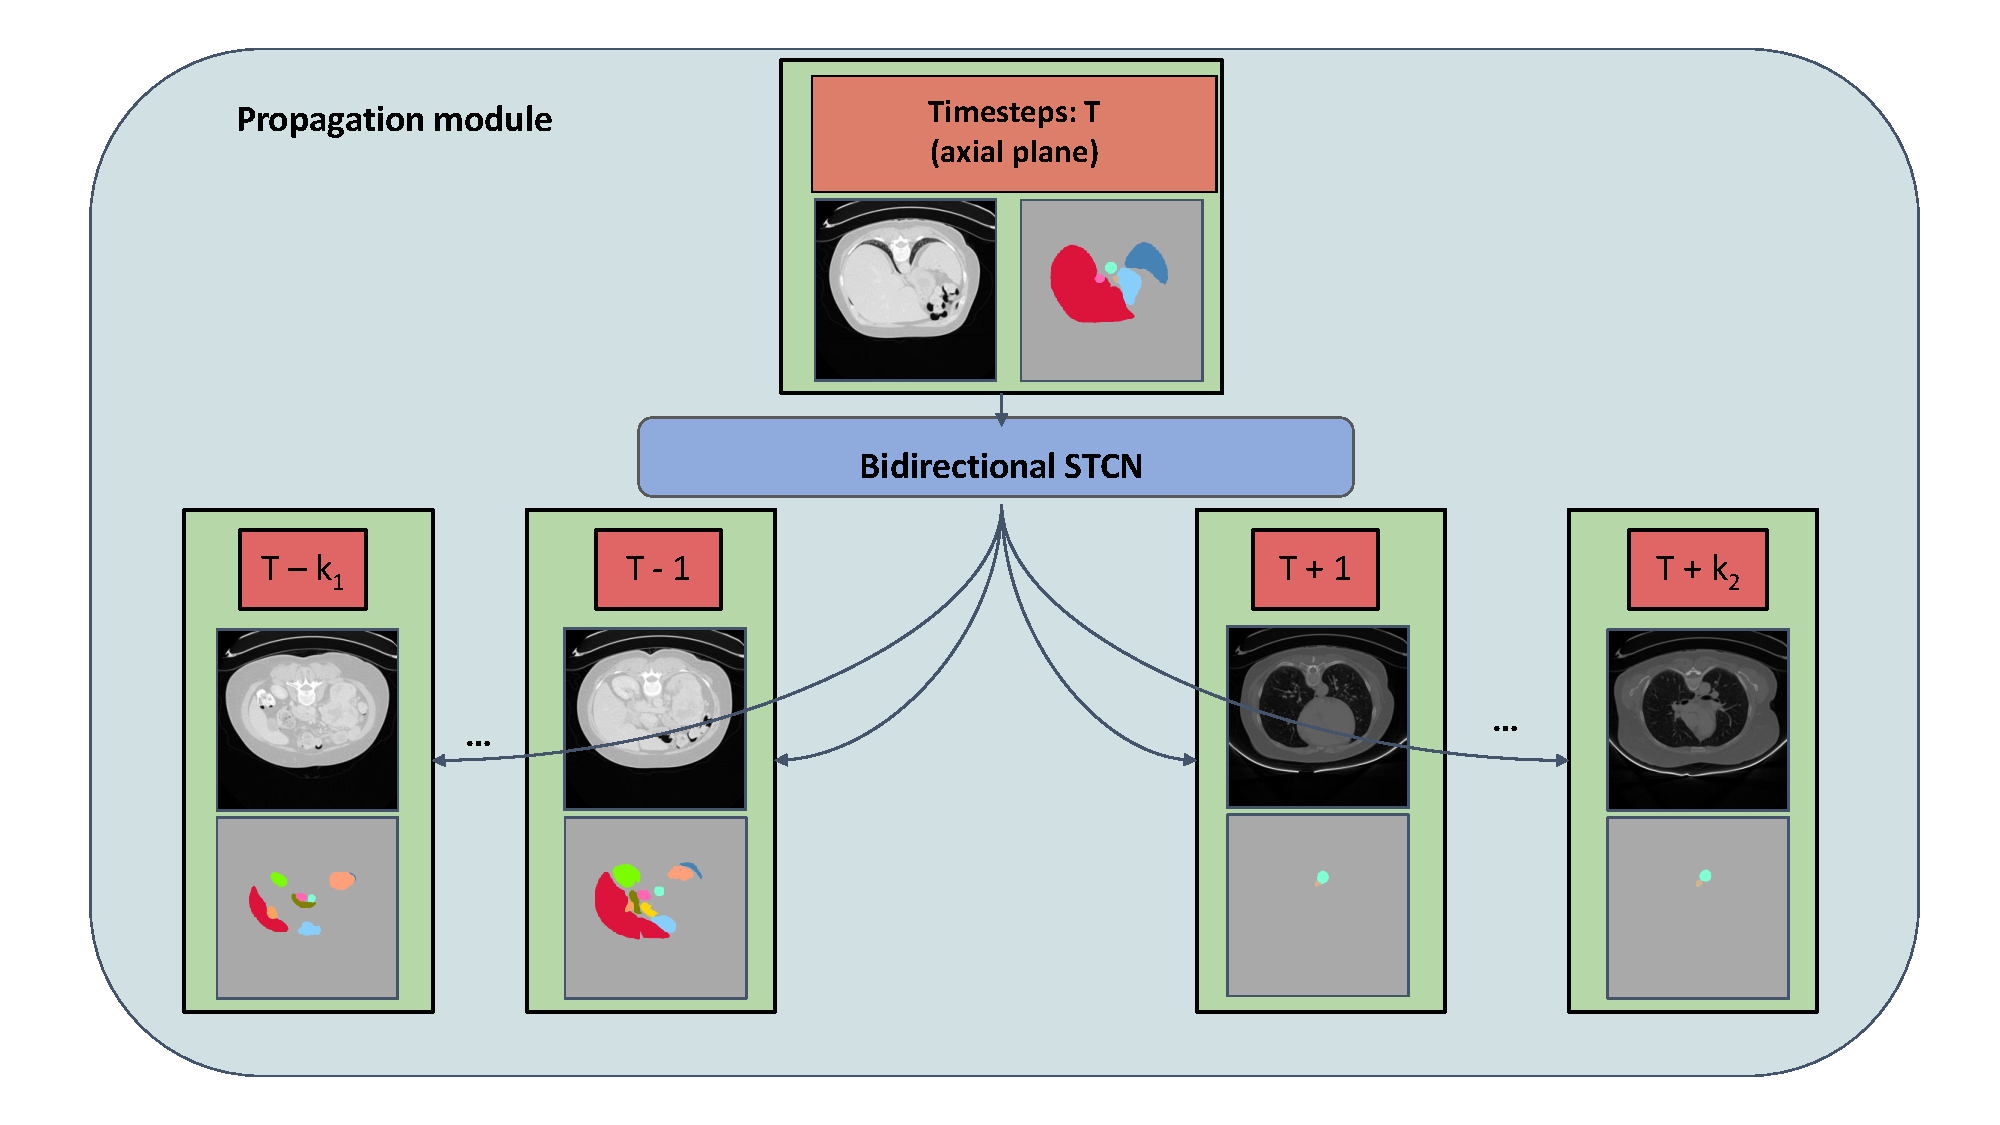
\includegraphics[width=\textwidth]{content/resources/new_images/propagation.pdf}
%     \caption{The propagation module. From an annotated slice of CT, at timestep T, STCN can make use of that to spread the information through the entire defined range $[T-k_1, T+k_2]$.}
%     \label{fig:labeling}
% \end{figure}


Given a vast amount of unlabeled CT volumes, we apply a uncertainty estimation technique to effectively maximize the utilization of the data.

Firstly, several CPS models are trained on the provided labeled data.
Then, we use these trained CPS models to obtain pseudo masks on the unlabeled set. Inspired from \cite{wang2019active}, we calculate the dice scores between these pseudo masks and the aggregated one. The mean of these dice scores will be compared with a threshold to determine whether the aggregated pseudo masks are qualified. Simply speaking, consensus-based assessment is used to evaluate the quality of pseudo labels.

We determine a single score for the $i^{th}$ volume in the unlabeled set as the formulation below:

\begin{align}
        score_{i} &= \frac{1}{K \times M} \sum_{k=1}^{K^{i}} \sum_{m=1}^{M} \text{DSC}(\mathcal{Y}^{k,i}_{m}, \mathcal{Y}^{k,i}_{AVG}) \\
        \text{dsc}  &= \frac{2 |X \cap Y|}{|X| + |Y|}
\end{align}

DSC represents the Dice Score evaluation metric calculating the overlapping area of prediction $X$ and ground truth $Y$. 
Here $\mathcal{Y}^{k,i}_{m}$ indicates the $m^{th}$ model’s output of the $k^{th}$ slice of volume $i$ while $\mathcal{Y}^{k,i}_{AVG}$ is the mask averaged from all $M$ models for the same slice. The easier the sample is, the more inclined the segmentation are to get a similar output if the sample is easier. In contrast, hard samples are more likely to be segmented differently by different models. Hence, we use the proposed score to measure the certainty between models' predictions. Higher score gives more credibility to the prediction, as it is more consistent. 

All aggregated samples that have high certainty are then reused for the next supervised training cycle. And after the training finishes, the same labeling process is repeated until all aforementioned models achieve satisfied performance or every unlabeled data has been used.